
\begin{align}
\because     \vec{A} = b\myvec{\cos C\\ \sin C}, \vec{B} = \myvec{a\\0}, \vec{C} = \myvec{0\\0},
    \end{align}
    substituting the given values, 
    \begin{align}
        \vec{A} = 5\myvec{\cos60\\ \sin60} = \myvec{2.5\\2.5\sqrt3},  \vec{B} = \myvec{7.5\\0},  \vec{C} = \myvec{0\\0}
        \end{align}
    which are plotted in Fig. \ref{constr/july/2Figure}.       

\begin{figure}[!h]
         \centering
         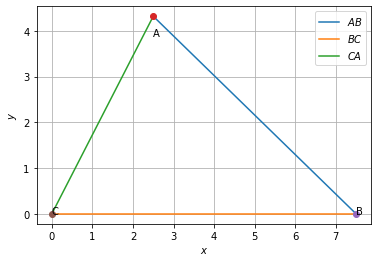
\includegraphics[width= \columnwidth]{solutions/july/2/2/Figures/Figure 1.png}
         \caption{The Constructed triangle}
         \label{constr/july/2Figure}
\end{figure}



